\documentclass[12pt, spanish]{article}
\usepackage[spanish]{babel}
\selectlanguage{spanish}
%\usepackage{natbib}
\usepackage{url}
\usepackage[utf8]{inputenc}
\usepackage{graphicx}
\graphicspath{{images/}}
\usepackage{parskip}
\usepackage{fancyhdr}
\usepackage{vmargin}
\usepackage{multirow}
\usepackage{float}
\usepackage{chngpage}

\usepackage{amsfonts}

\usepackage{subcaption}

\usepackage{hyperref}
\usepackage[
    type={CC},
    modifier={by-nc-sa},
    version={4.0},
]{doclicense}

\hypersetup{
    colorlinks=true,
    linkcolor=blue,
    filecolor=magenta,
    urlcolor=cyan,
}

% para codigo
\usepackage{listings}
\usepackage{xcolor}



%% configuración de listings

\definecolor{listing-background}{HTML}{F7F7F7}
\definecolor{listing-rule}{HTML}{B3B2B3}
\definecolor{listing-numbers}{HTML}{B3B2B3}
\definecolor{listing-text-color}{HTML}{000000}
\definecolor{listing-keyword}{HTML}{435489}
\definecolor{listing-identifier}{HTML}{435489}
\definecolor{listing-string}{HTML}{00999A}
\definecolor{listing-comment}{HTML}{8E8E8E}
\definecolor{listing-javadoc-comment}{HTML}{006CA9}

\lstdefinestyle{eisvogel_listing_style}{
  language         = python,
%$if(listings-disable-line-numbers)$
%  xleftmargin      = 0.6em,
%  framexleftmargin = 0.4em,
%$else$
  numbers          = left,
  xleftmargin      = 0em,
 framexleftmargin = 0em,
%$endif$
  backgroundcolor  = \color{listing-background},
  basicstyle       = \color{listing-text-color}\small\ttfamily{}\linespread{1.15}, % print whole listing small
  breaklines       = true,
  frame            = single,
  framesep         = 0.19em,
  rulecolor        = \color{listing-rule},
  frameround       = ffff,
  tabsize          = 4,
  numberstyle      = \color{listing-numbers},
  aboveskip        = 1.0em,
  belowskip        = 0.1em,
  abovecaptionskip = 0em,
  belowcaptionskip = 1.0em,
  keywordstyle     = \color{listing-keyword}\bfseries,
  classoffset      = 0,
  sensitive        = true,
  identifierstyle  = \color{listing-identifier},
  commentstyle     = \color{listing-comment},
  morecomment      = [s][\color{listing-javadoc-comment}]{/**}{*/},
  stringstyle      = \color{listing-string},
  showstringspaces = false,
  escapeinside     = {/*@}{@*/}, % Allow LaTeX inside these special comments
  literate         =
  {á}{{\'a}}1 {é}{{\'e}}1 {í}{{\'i}}1 {ó}{{\'o}}1 {ú}{{\'u}}1
  {Á}{{\'A}}1 {É}{{\'E}}1 {Í}{{\'I}}1 {Ó}{{\'O}}1 {Ú}{{\'U}}1
  {à}{{\`a}}1 {è}{{\'e}}1 {ì}{{\`i}}1 {ò}{{\`o}}1 {ù}{{\`u}}1
  {À}{{\`A}}1 {È}{{\'E}}1 {Ì}{{\`I}}1 {Ò}{{\`O}}1 {Ù}{{\`U}}1
  {ä}{{\"a}}1 {ë}{{\"e}}1 {ï}{{\"i}}1 {ö}{{\"o}}1 {ü}{{\"u}}1
  {Ä}{{\"A}}1 {Ë}{{\"E}}1 {Ï}{{\"I}}1 {Ö}{{\"O}}1 {Ü}{{\"U}}1
  {â}{{\^a}}1 {ê}{{\^e}}1 {î}{{\^i}}1 {ô}{{\^o}}1 {û}{{\^u}}1
  {Â}{{\^A}}1 {Ê}{{\^E}}1 {Î}{{\^I}}1 {Ô}{{\^O}}1 {Û}{{\^U}}1
  {œ}{{\oe}}1 {Œ}{{\OE}}1 {æ}{{\ae}}1 {Æ}{{\AE}}1 {ß}{{\ss}}1
  {ç}{{\c c}}1 {Ç}{{\c C}}1 {ø}{{\o}}1 {å}{{\r a}}1 {Å}{{\r A}}1
  {€}{{\EUR}}1 {£}{{\pounds}}1 {«}{{\guillemotleft}}1
  {»}{{\guillemotright}}1 {ñ}{{\~n}}1 {Ñ}{{\~N}}1 {¿}{{?`}}1
  {…}{{\ldots}}1 {≥}{{>=}}1 {≤}{{<=}}1 {„}{{\glqq}}1 {“}{{\grqq}}1
  {”}{{''}}1
}
\lstset{style=eisvogel_listing_style}


\usepackage[default]{sourcesanspro}

\setmarginsrb{2 cm}{1 cm}{2 cm}{2 cm}{1 cm}{1.5 cm}{1 cm}{1.5 cm}

\title{Entrega final:\\
Estado actual del proyecto.\hspace{0.05cm} }
\author{Guillermo Sandoval Schmidt\\ Antonio David Villegas Yeguas}
\date{\today}

\makeatletter
\let\thetitle\@title
\let\theauthor\@author
\let\thedate\@date
\makeatother

\pagestyle{fancy}
\fancyhf{}
\rhead{\theauthor}
\lhead{\thetitle}
\cfoot{\thepage}

\begin{document}

%%%%%%%%%%%%%%%%%%%%%%%%%%%%%%%%%%%%%%%%%%%%%%%%%%%%%%%%%%%%%%%%%%%%%%%%%%%%%%%%%%%%%%%%%

\begin{titlepage}
    \centering
    \vspace*{0.3 cm}
    
\includegraphics[scale = 0.50]{ugr.png}\\[0.7 cm]
    %\textsc{\LARGE Universidad de Granada}\\[2.0 cm]
    \textsc{\large 4º CSI 2020/21}\\[0.5 cm]
    \textsc{\large Grado en Ingeniería Informática}\\[0.5 cm]
    \rule{\linewidth}{0.2 mm} \\[0.2 cm]
    { \huge \bfseries \thetitle}\\
    \rule{\linewidth}{0.2 mm} \\[1 cm]

    \begin{minipage}{0.4\textwidth}
        \begin{flushleft} \large
            \emph{Autores:}\\
            \theauthor\\
            \end{flushleft}
            \end{minipage}~
            \begin{minipage}{0.4\textwidth}
            \begin{flushright} \large
            \emph{Asignatura: \\
            Programación Lúdica}   \\
        \end{flushright}
    \end{minipage}\\[0.5cm]

    {\large \thedate}\\[0.5cm]
    %{\url{https://github.com/advy99/AA/}}
    {\doclicenseThis}

    \vfill

\end{titlepage}

%%%%%%%%%%%%%%%%%%%%%%%%%%%%%%%%%%%%%%%%%%%%%%%%%%%%%%%%%%%%%%%%%%%%%%%%%%%%%%%%%%%%%%%%%

\tableofcontents
\pagebreak

%%%%%%%%%%%%%%%%%%%%%%%%%%%%%%%%%%%%%%%%%%%%%%%%%%%%%%%%%%%%%%%%%%%%%%%%%%%%%%%%%%%%%%%%%

\section{Integrantes del grupo}

Los integrantes del grupo somos:

\begin{itemize}
	\item Guillermo Sandoval Schmidt
	\item Antonio David Villegas Yeguas
\end{itemize}

\section{Propuesta}

\subsection{Título provisional}

Como título provisional hemos decidido \textbf{Lose to Win}, debido a la principal mecánica del videojuego que explicaremos en la descripción.

\subsection{Descripción del juego, género y público objetivo}


Lose to Win es un juego multijugador de partidas rápidas basado en minijuegos, donde los jugadores se enfrentan todos contra todos o por equipos para alzarse con la victoria.

Cuenta con una mecánica transversal a los diversos minijuegos, ya que para ganar debes perder el minijuego.

Algunos de los minijuegos que hemos pensado son:

\begin{enumerate}
	\item Bomb tag: uno de los jugadores aparece con una bomba, al tocar al jugador con la bomba se la robas. Gana el jugador que tenga la bomba cuando explote.
	\item Egg Giver: el clásico juego de coger huevos y llevarlos a tu base pero al revés, gana el jugador que menos huevos tenga en su base.
	\item Spike Ball: similar al minijuego de “Move or Die” de mismo nombre, pero el objetivo es que la bola de pinchos te mate, ganando el jugador que más veces muera.
	\item Generous Guy: recoge objetos del color del rival para que gane puntos y ganar siendo el jugador con menos puntos.
\end{enumerate}


Nuestra idea no se encaja en un único género, debido a la gran variedad de minijuegos y objetivos de las distintas partidas, aun así, los principales géneros de nuestra idea serían acción, party game y plataformas.

En principio el público objetivo sería cualquier persona, independientemente de la edad (PEGI 3), aunque es cierto que esto variará dependiendo del estilo gráfico del juego y como de explícito sea con respecto a la violencia de los minijuegos, tanto a nivel de que tipos de minijuegos como a nivel artístico, lo que conllevaría un PEGI 12.

\section{Estudio de mercado}

Aunque hemos encontrado una gran cantidad de videojuegos similares a nuestra idea, finalmente hemos escogido estos tres ya que son los más parecidos a nuestra propuesta.

\subsection{Move or Die}

Se trata de un videojuego para cuatro jugadores en el que cada jugador controla un personaje cuya vida se reduce rápidamente si el jugador deja de moverse por un momento, se regenerá si reanuda el movimiento. Cada ronda contará con distintas reglas o modificadores, que varían entre los distintos modos. El desafío surge cuando los jugadores siguen moviéndose para ganar, mientras evitan peligros como picos o bloques que caen. Los jugadores también pueden empujarse entre sí.


\subsubsection{Detalles sobre el videojuego}

\begin{itemize}
	\item \textbf{Compañia}: Those Awesome Guys
	\item \textbf{Plataformas}: Windows, Linux, macOS, PlayStation 4
	\item \textbf{Modelo de negocio}: Juego de pago (Pay-to-play)
	\item \textbf{Web}: \url{http://www.moveordiegame.com}
\end{itemize}

\subsubsection{Capturas del videojuego}

\begin{figure}[H]
  \centering
   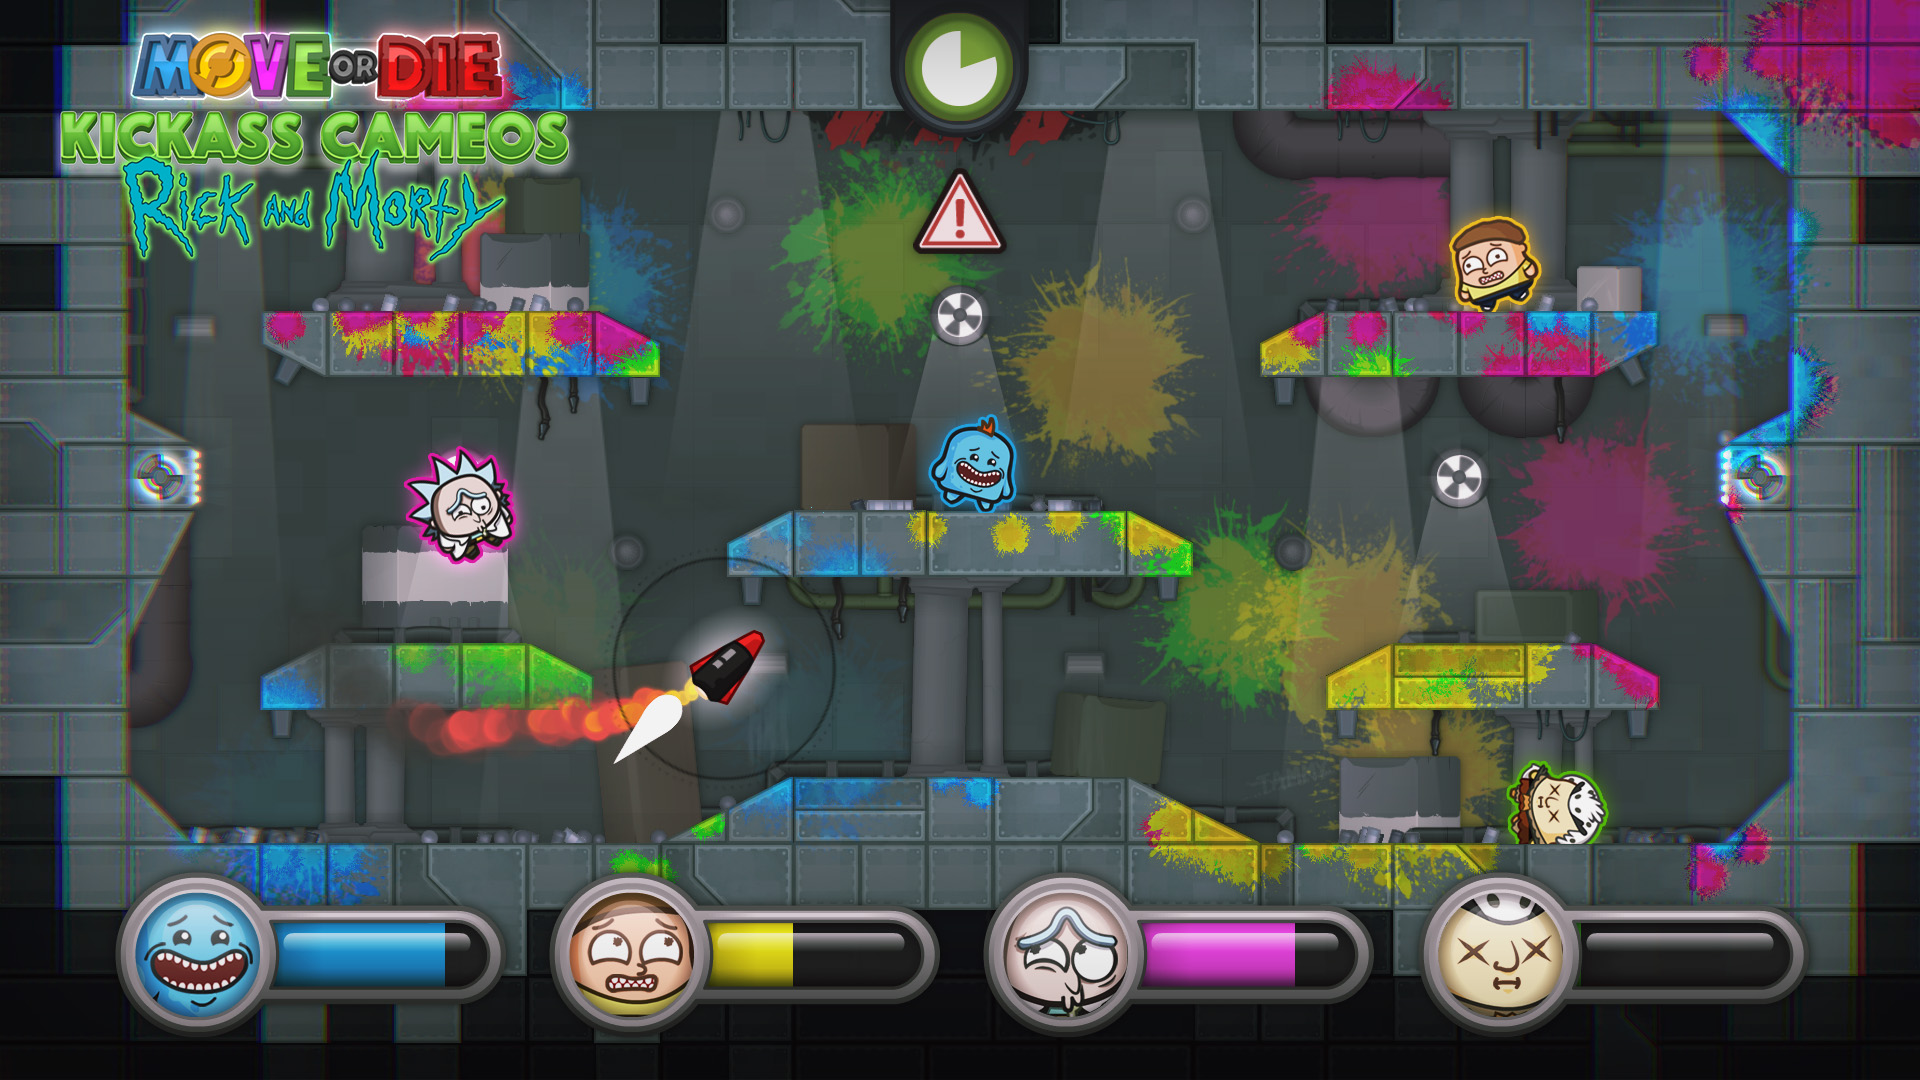
\includegraphics[width=\textwidth]{mod_juego.jpg}
	\caption{Imagen de Move or Die dentro de una partida.}
\end{figure}

\begin{figure}[H]
  \centering
   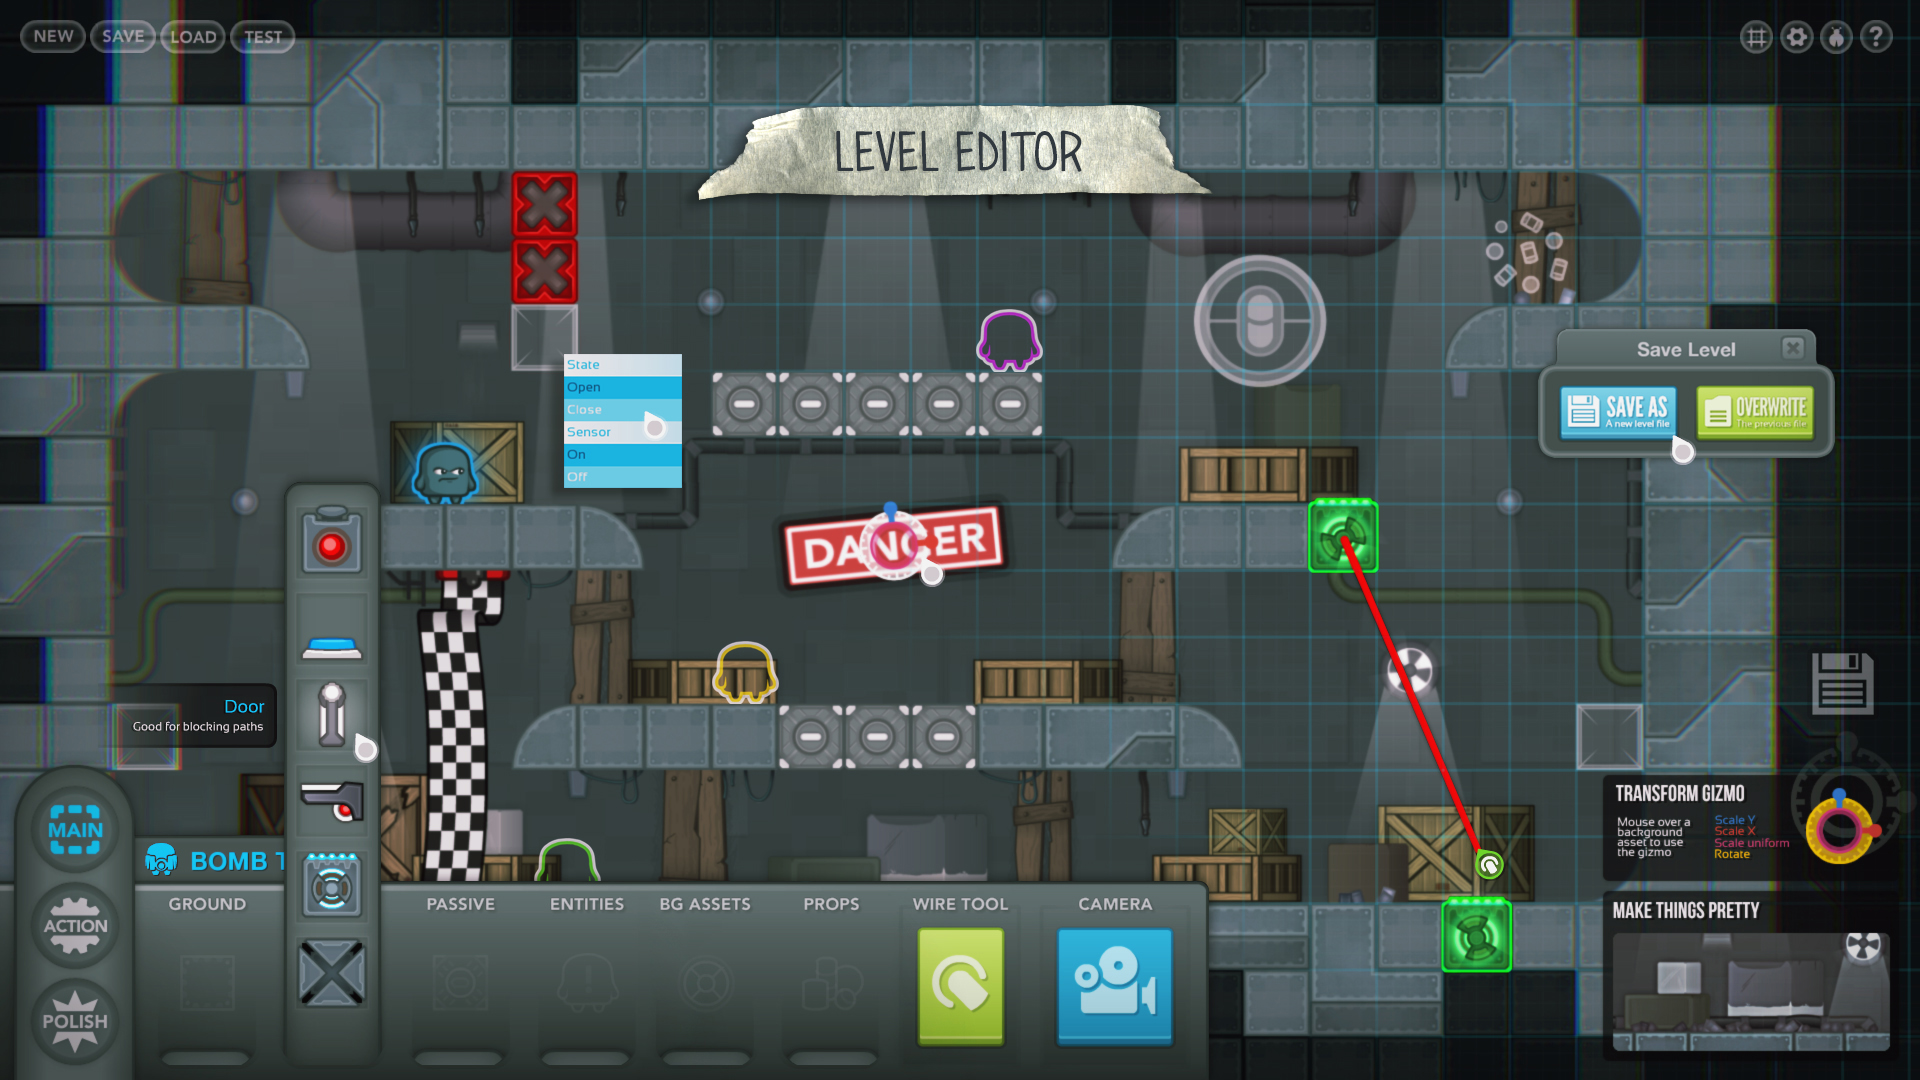
\includegraphics[width=\textwidth]{mod_editor.jpg}
	\caption{Editor de niveles de Move or Die.}
\end{figure}

\begin{figure}[H]
  \centering
   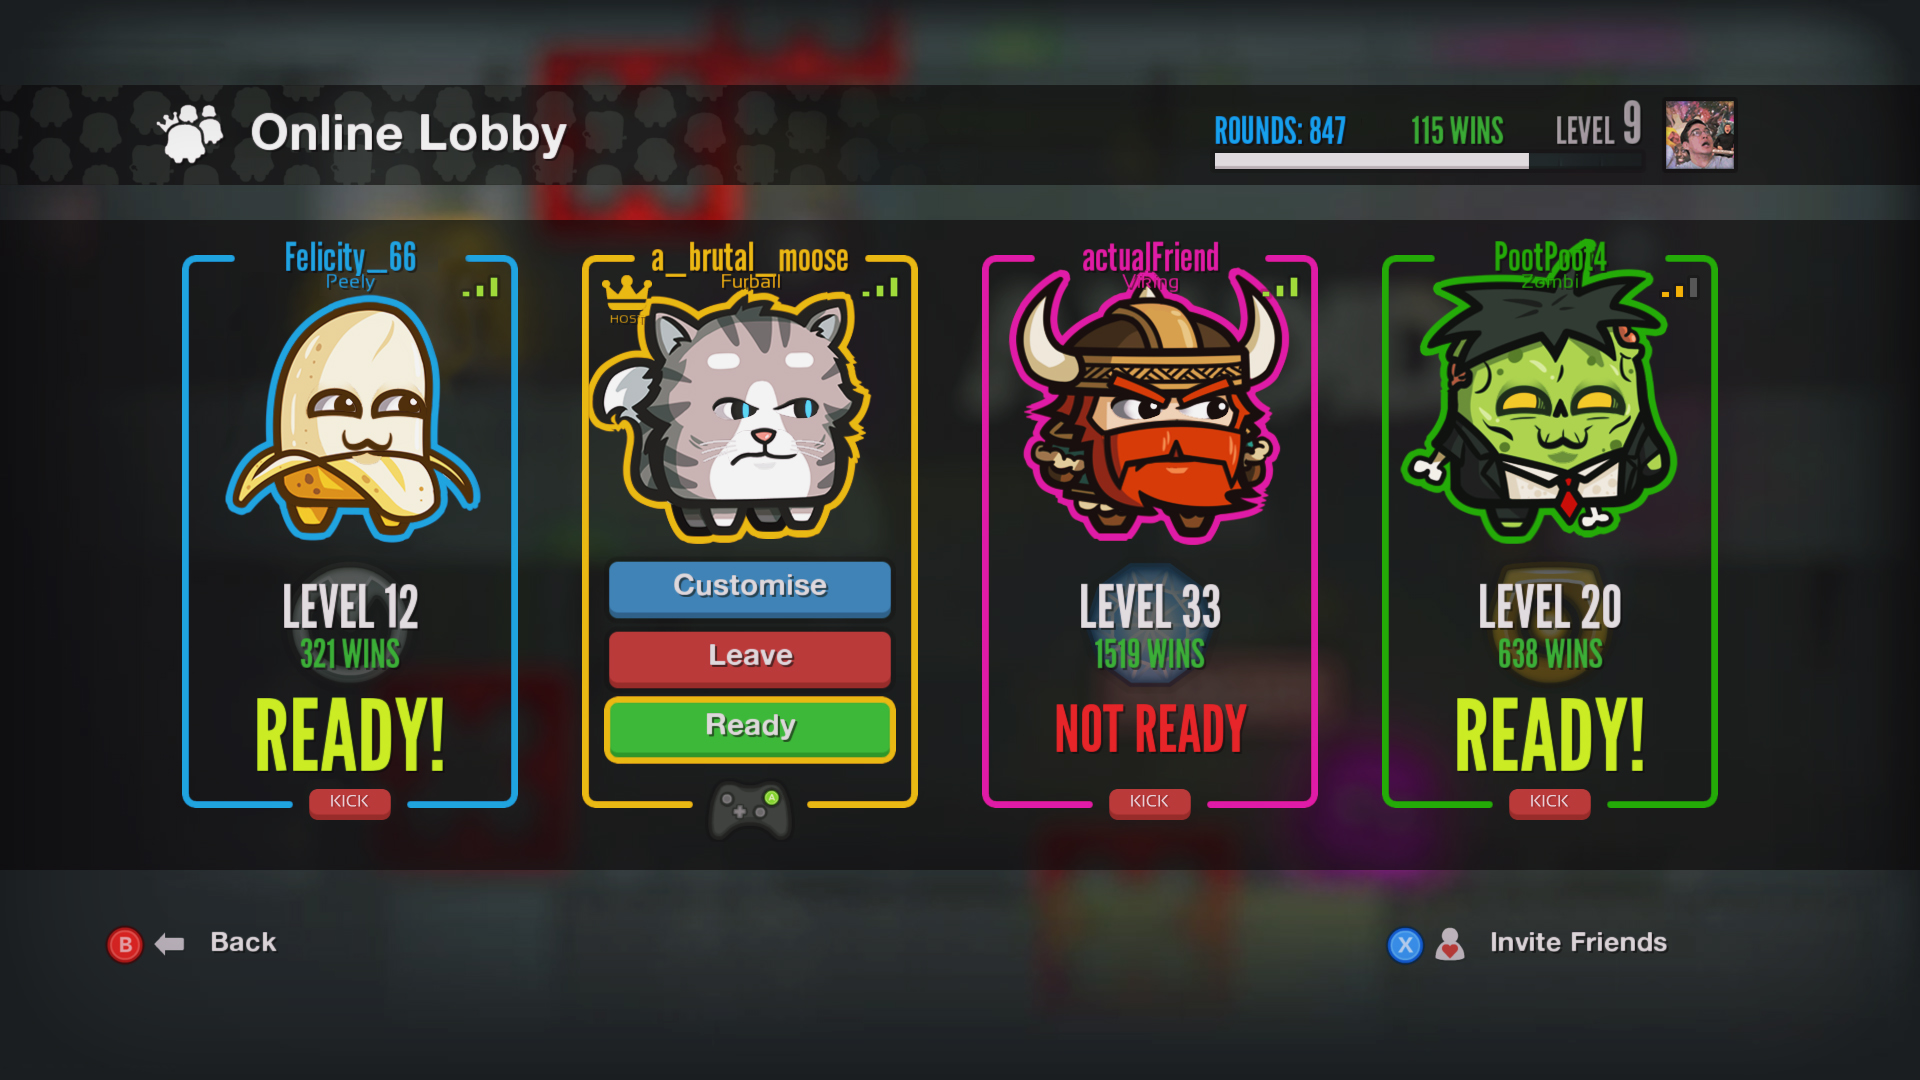
\includegraphics[width=\textwidth]{mod_lobby.jpg}
	\caption{Lobby de Move or Die.}
\end{figure}

\subsubsection{Aspectos positivos}

\begin{itemize}
	\item Juego local y online.
	\item De 1 a 4 jugadores.
	\item Incluye editor de niveles.
	\item Facilidad para crear mods.
	\item Compatible con mando y teclado.
	\item Juego multiplataforma (puedes jugar con una persona que no esté jugando en tu misma plataforma).
	\item Variedad de minijuegos.
\end{itemize}

\subsubsection{Aspectos negativos}

\begin{itemize}
	\item Requiere muchas horas desbloquear los distintos modos de juego.
	\item Modos de juego bloqueados que solo se pueden desbloquear con “monedas del juego”.
	\item Malos servidores para jugar online.
\end{itemize}

\subsection{Party Panic}

Es un juego multijugador de hasta cuatro jugadores en el que compiten unos contra otros en distintos minijuegos. Gana el jugador que más minijuegos complete victorioso.

\subsubsection{Detalles sobre el videojuego}

\begin{itemize}
	\item \textbf{Compañia}: Everglow Interactive
	\item \textbf{Plataformas}: Windows, macOS, Linux, XBOX ONE, PlayStation 4
	\item \textbf{Modelo de negocio}: Juego de pago (Pay-to-play)
	\item \textbf{Web}: \url{https://partypanicgame.com/}
\end{itemize}

\subsubsection{Capturas del videojuego}


\begin{figure}[H]
  \centering
   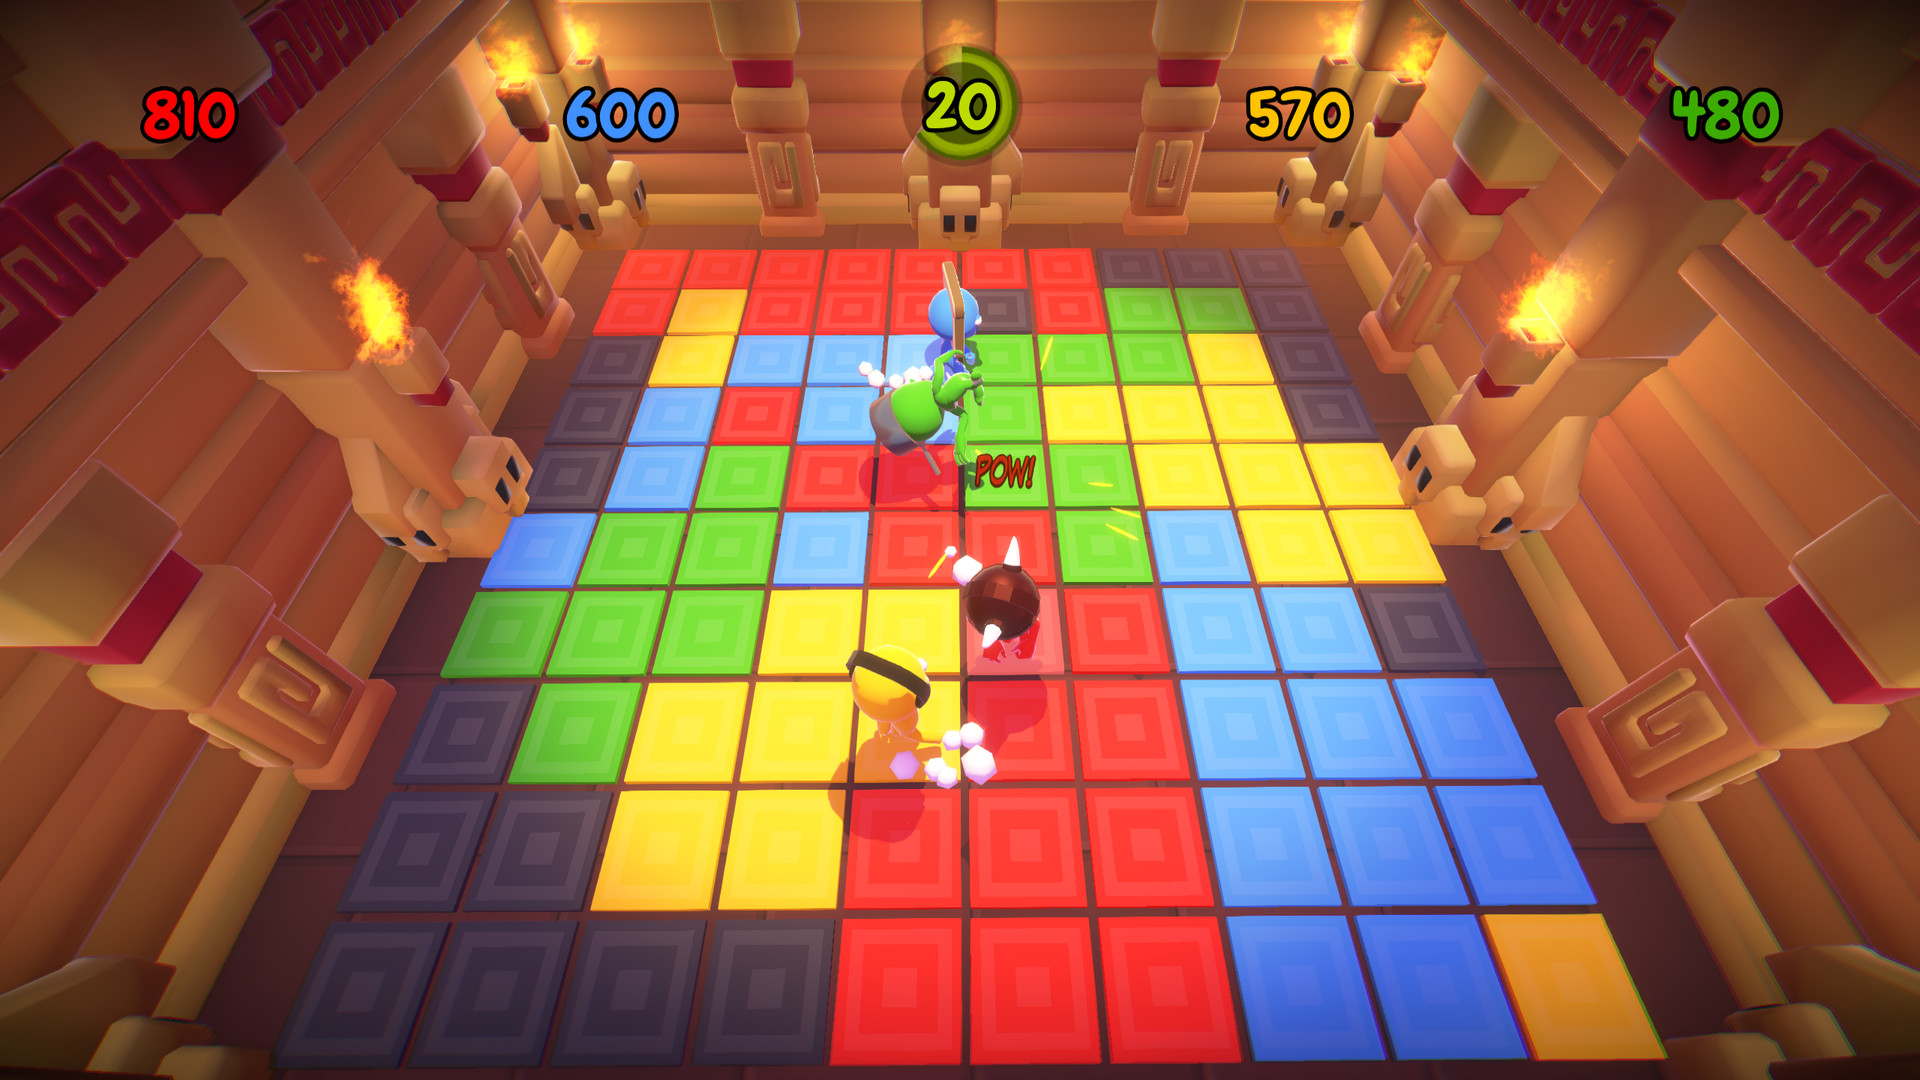
\includegraphics[width=\textwidth]{pp_juego.jpg}
	\caption{Imagen de Party Panic dentro de una partida.}
\end{figure}

\begin{figure}[H]
  \centering
   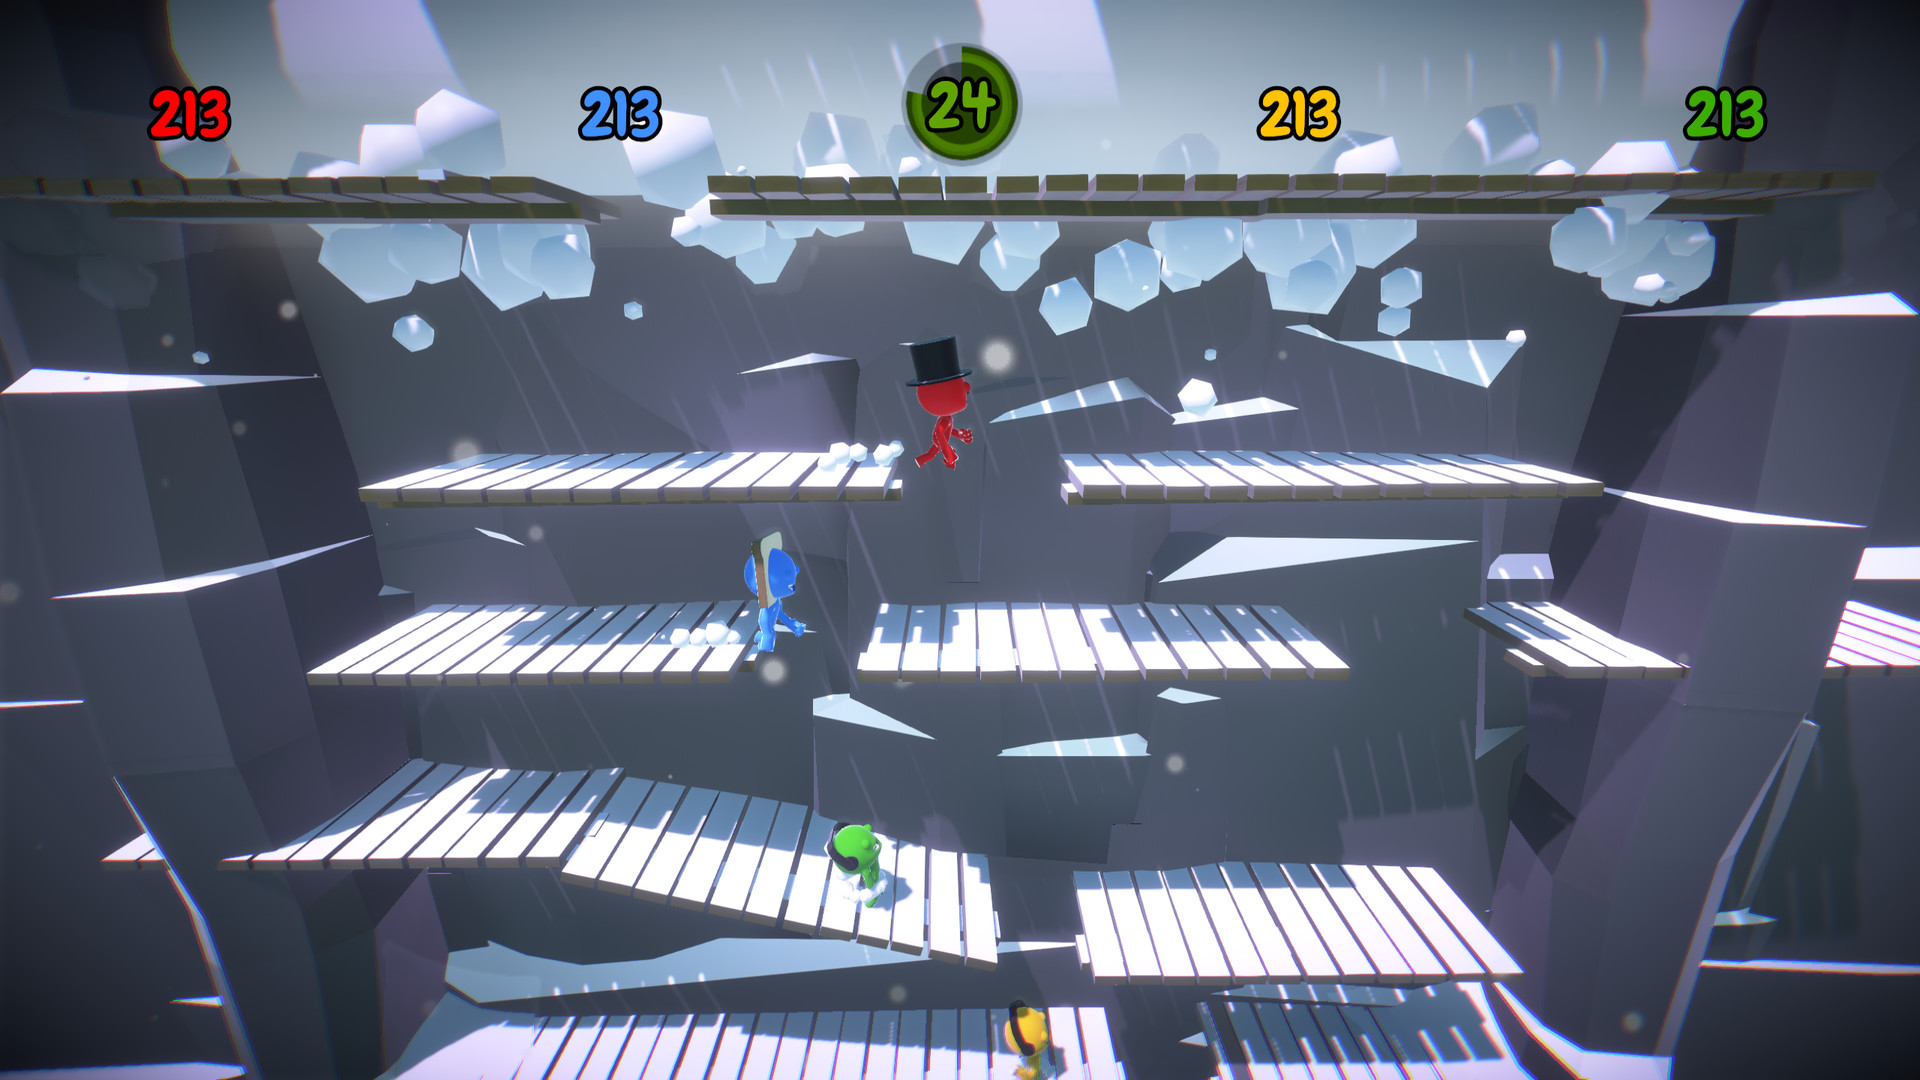
\includegraphics[width=\textwidth]{pp_juego2.jpg}
	\caption{Imagen de Party Panic dentro de una partida.}
\end{figure}


\begin{figure}[H]
  \centering
   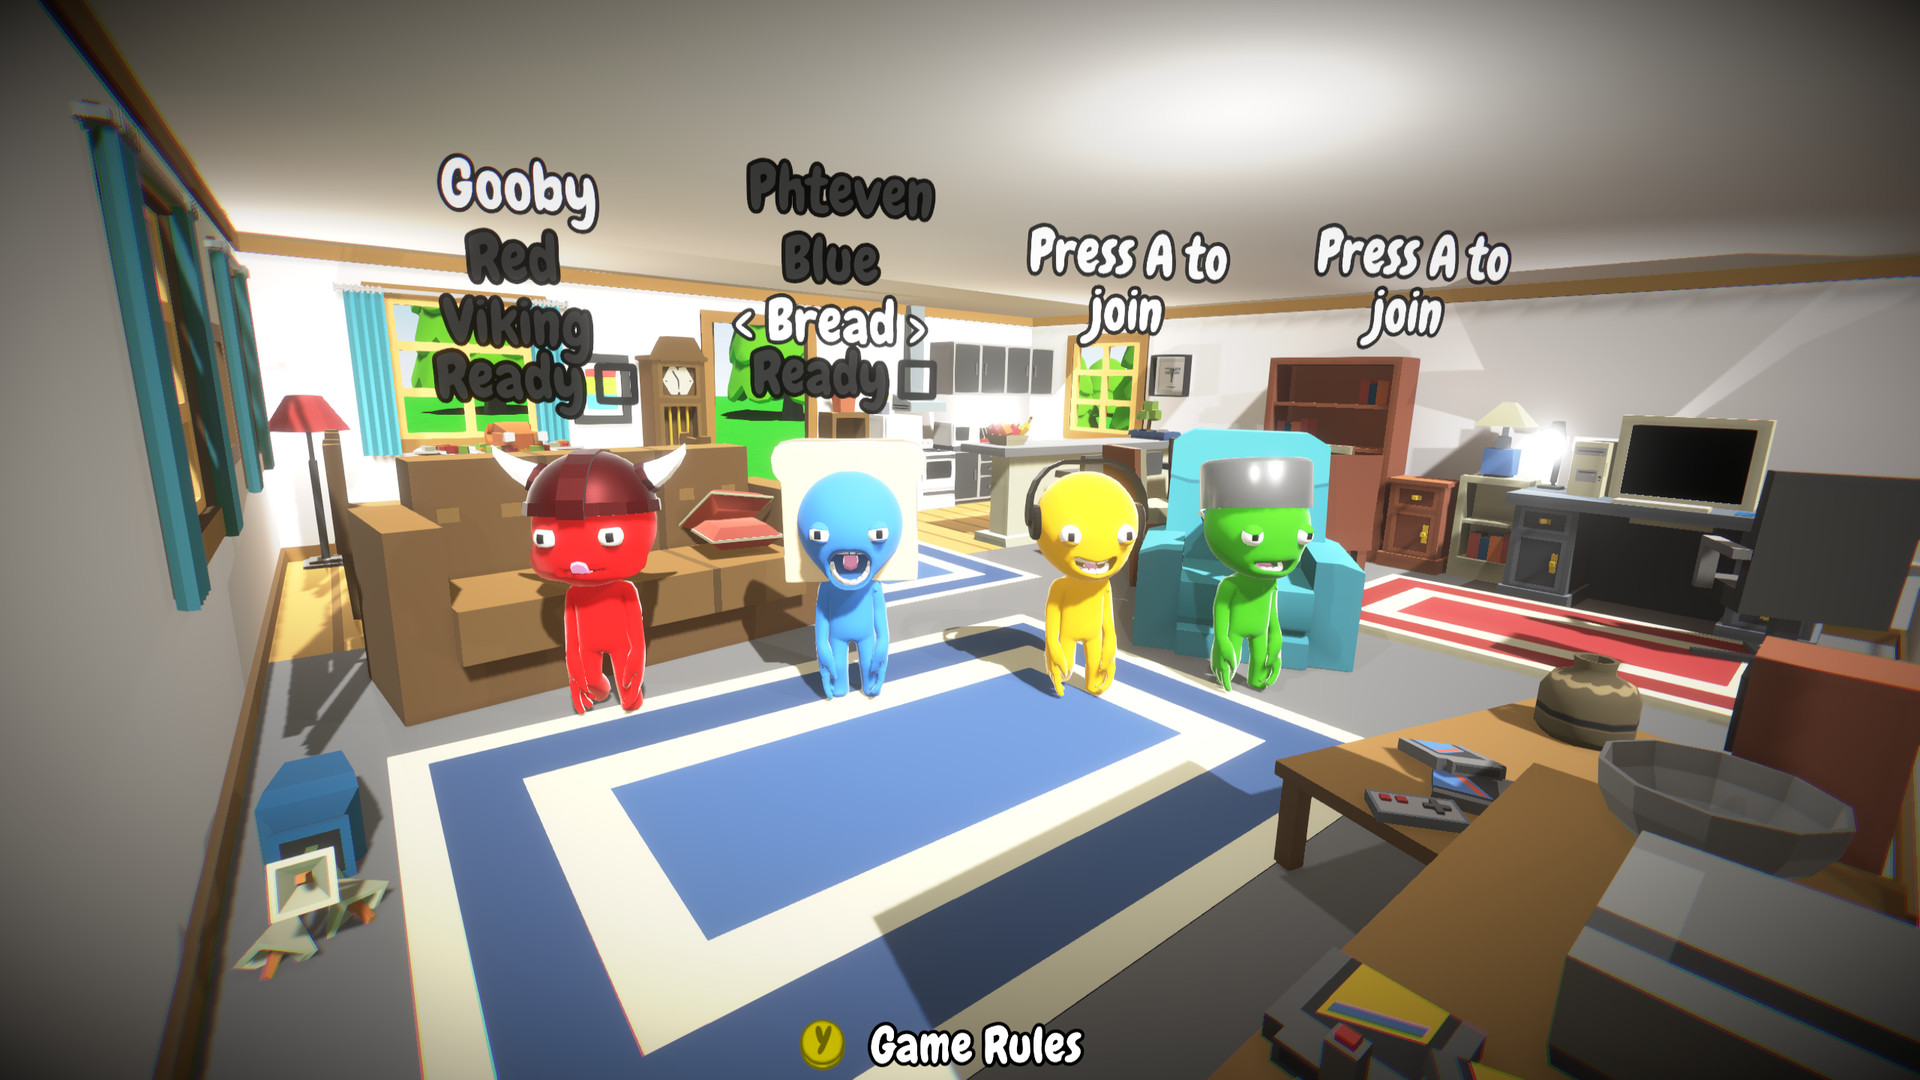
\includegraphics[width=\textwidth]{pp_lobby.jpg}
	\caption{Lobby de Party Panic.}
\end{figure}

\subsubsection{Aspectos positivos}

\begin{itemize}
	\item Juego local y online.
	\item De 1 a 4 jugadores.
	\item Compatible con mando y teclado.
\end{itemize}

\subsubsection{Aspectos negativos}

\begin{itemize}
	\item No tiene editor de niveles ni soporte de mods.
	\item La IA no funciona correctamente.
	\item Interfaz muy básica y poco accesible.
	\item En una partida no se permiten jugadores de distintas plataformas.
	\item Falta variedad de jugadores.
	\item Malos servidores.
\end{itemize}

\subsection{Duck Game}

Es un videojuego de acción donde los personajes son patos que incluye características de videojuegos de disparos y plataformas. El juego tiene un modo de un jugador al igual que un modo multijugador en línea con un límite de hasta siete jugadores más. En este modo de juego el jugador que reciba un solo disparo muere y el jugador sobreviviente gana la ronda.


\subsubsection{Detalles sobre el videojuego}

\begin{itemize}
	\item \textbf{Compañia}: Adult Swim Games
	\item \textbf{Plataformas}: Windows, PlayStation 4, Switch
	\item \textbf{Modelo de negocio}: Juego de pago (Pay-to-play)
	\item \textbf{Web}: \url{https://www.adultswim.com/games/duck-game}
\end{itemize}

\subsubsection{Capturas del videojuego}

\begin{figure}[H]
  \centering
   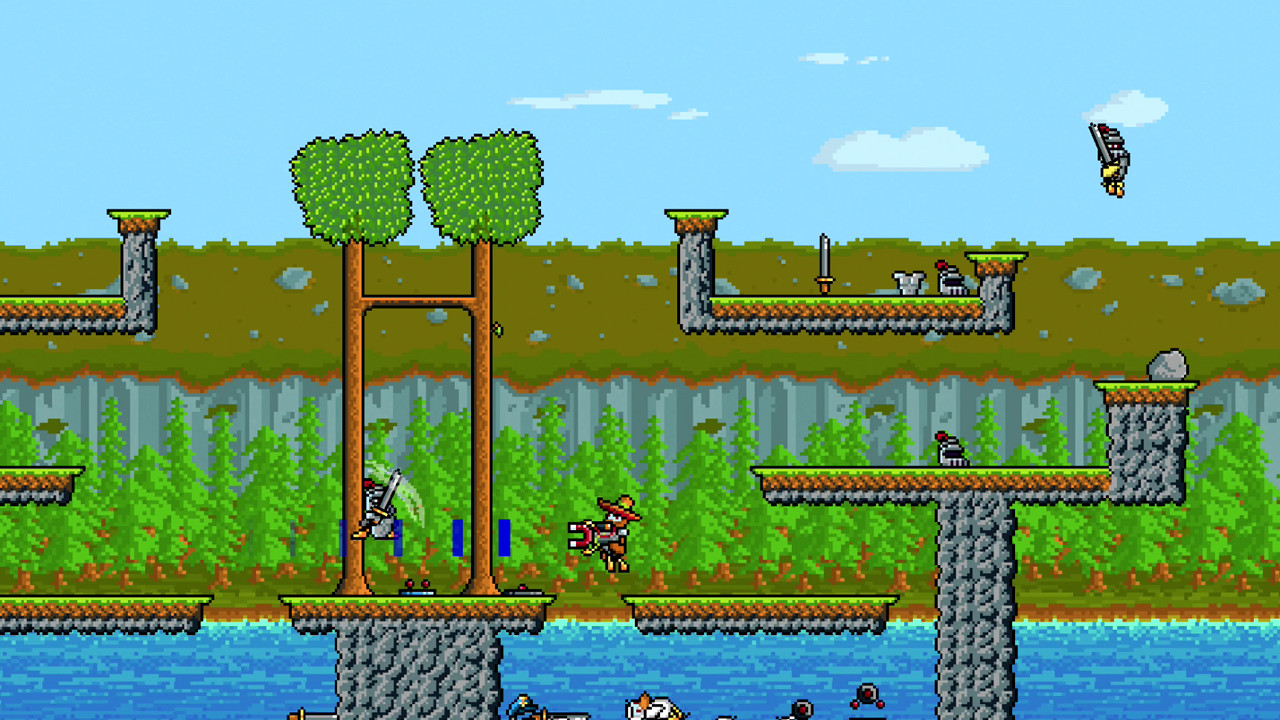
\includegraphics[width=\textwidth]{dg_juego.jpg}
	\caption{Imagen de una partida de Duck Game.}
\end{figure}

\begin{figure}[H]
  \centering
   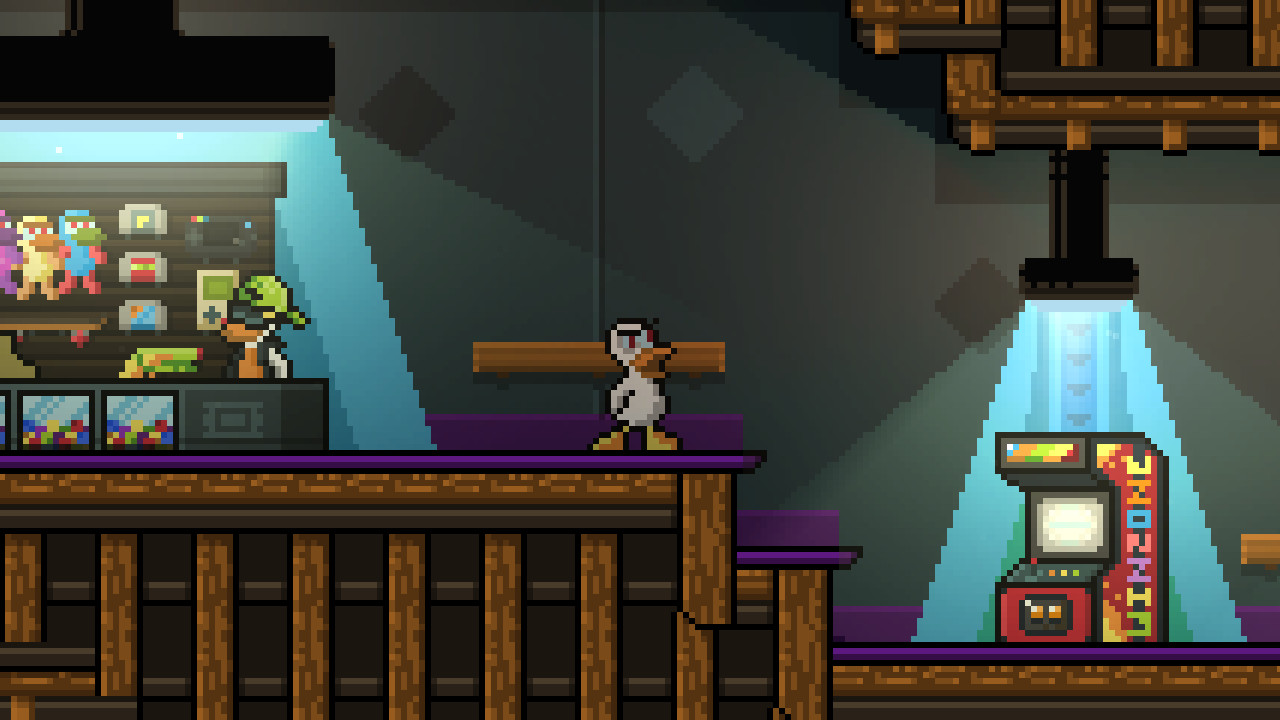
\includegraphics[width=\textwidth]{dg_muestra.jpg}
	\caption{Imagen de una escena de Duck Game.}
\end{figure}


\begin{figure}[H]
  \centering
   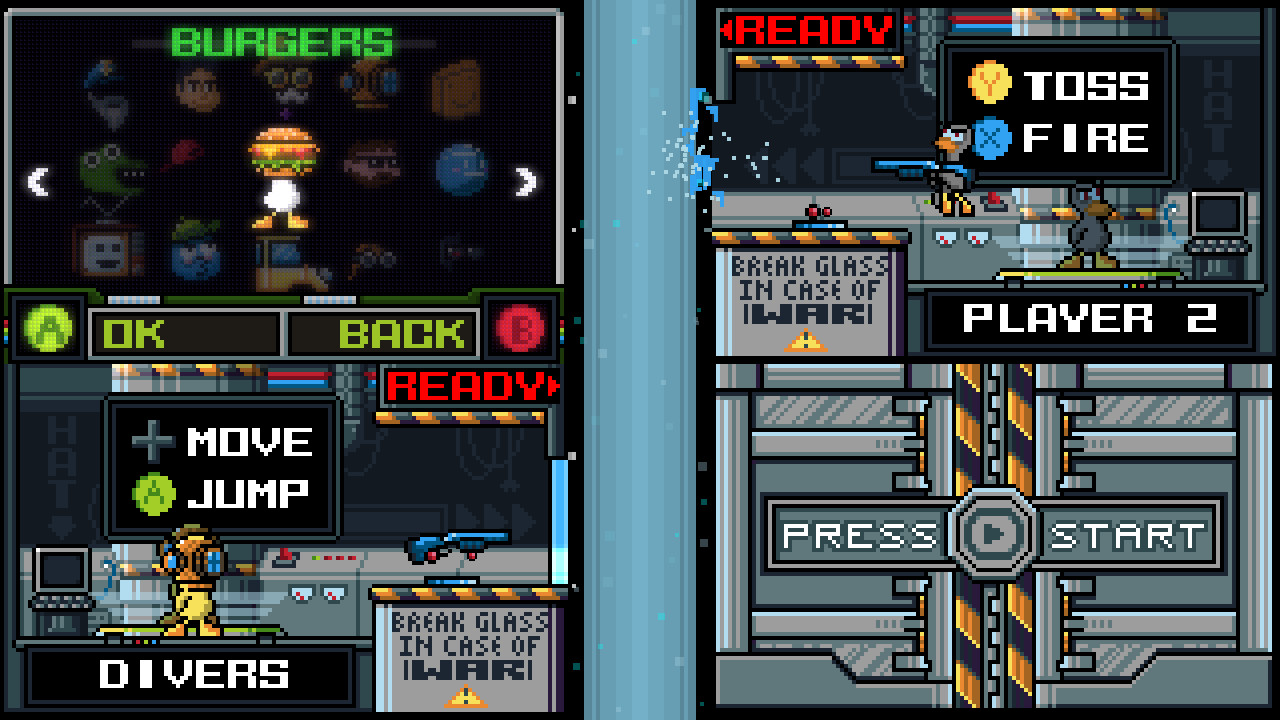
\includegraphics[width=\textwidth]{dg_lobby.jpg}
	\caption{Lobby de Duck Game.}
\end{figure}

\subsubsection{Aspectos positivos}

\begin{itemize}
	\item Juego local y online.
	\item De 2 a 8 jugadores.
	\item Incluye editor de niveles.
	\item Compatible con mando y teclado.
	\item En una partida no se permiten jugadores de distintas plataformas.
\end{itemize}

\subsubsection{Aspectos negativos}

\begin{itemize}
	\item Malos servidores.
	\item No permite modificar el esquema de control.
	\item No permite utilizar múltiples mandos en juego local.
	\item No permite permite varios jugadores
\end{itemize}


\end{document}
